\chapter{Critical Assessment}
\label{chap:assessment}

%##################################################################################################
\section{Chapter Overview}
%##################################################################################################

In Chapter~\ref{chap:introduction}, I listed six original contributions made by my doctoral work. Having now discussed the work underlying the contributions in detail in the preceding chapters, and validated my feature identification work in the previous chapter, the goal of this chapter is to evaluate the usefulness of these contributions both within the context of my doctorate and (where applicable) more widely.

%##################################################################################################
\section{Partition Forest Algorithms}
%##################################################################################################

In \S\ref{sec:ipfs-mutatingalgorithms}, I introduced a comprehensive set of algorithms for editing partition forests. Whilst partition forests themselves have appeared extensively in the imaging literature under a variety of different names (see \S\ref{subsec:background-partitionhierarchies-imagerepresentation}), little research attention has hitherto been devoted to the problem of editing them, with the notable exception of Nacken's work on parent switching (which he calls \emph{connectivity preserving relinking}) \cite{nacken95}. My algorithms as a whole thus fill a notable gap in the existing literature.

An ability to edit partition forests is useful in more than one domain. In image analysis, it allows a user to manage and make corrections to a hierarchical segmentation of an image, as demonstrated by my \emph{centipede} and \emph{millipede} segmentation tools. In hierarchical pathfinding, it allows nested partitions of a routing graph to be rearranged so as to minimise the memory consumed by statically-constructed pathfinding tables (this can be particularly important when developing a pathfinding solution that is to run on a machine with limited memory, such as a games console). In organising hierarchical teams of people (for instance, within a large organisation), it can be used to determine the effects of transferring a team member to another team -- will the original team fall apart because the person being transferred was the lynchpin holding things together?

The algorithms I have developed were designed to integrate particularly well into a graphical user interface. Even the more complex forest operations are undoable, and the algorithms all provide sufficient feedback on what changes they made to allow other parts of the program (such as the partition forest selection and the graphical representation of the partition forest) to react accordingly. Furthermore, all of the algorithms are efficient (as demonstrated by the complexity analysis in \S\ref{sec:ipfs-mutatingalgorithms}) and quick to execute in an interactive setting. The higher-level algorithms, such as non-sibling node merging and parent switching, are particularly helpful from the user's perspective, because they allow complicated forest operations to be performed with only a small amount of user interaction.

My parent switching algorithm itself is potentially an improvement on the one described by Nacken. As discussed in \S\ref{subsec:background-partitionhierarchies-imagerepresentation}, Nacken's approach allows the parent of a child to be switched only when both (a) the child is adjacent to a child of the new parent, and (b) moving the child will not affect the contiguity of the old parent. Whilst the first constraint is inherent, my algorithm circumvents the second constraint by splitting the old parent (and potentially some of its ancestors) where necessary, thus allowing further reasonable parent switches to be performed.

\iffalse
+ Useful both for imaging and hierarchical pathfinding
+ Algorithms carefully pinned down, well-justified, reasonable complexities
+ Parent switching algorithm improves on previous state-of-the-art (Nacken) because it makes extra reasonable parent switches possible
+ Unzipping, zipping, non-sibling node merging have no obvious comparisons in the literature
\fi

%##################################################################################################
\section{Partition Forest Selections}
%##################################################################################################

In \S\ref{sec:ipfs-selections}, I described a novel hierarchical representation for partition forest selections. This is based around the concept that the selection of an individual node in the forest equates to the selection of the subtree beneath it. It is a more compact representation than the obvious leaf-based representation that represents the selection as a set of selected partition forest leaves, and lends itself to more efficient interactive editing. For instance, if the user selects a high-level region in the partition forest and then wants to deselect one of its children, far fewer changes need to be made to the hierarchical representation than the leaf-based one (see Figure~\ref{fig:criticalassessment-selection-refinement}). It also avoids the problems that would be caused by an ad-hoc approach that allowed the user to simply add and remove individual nodes from a list of selected nodes. That approach fails because the representation in question admits the possibility of redundancy in the selection -- that is, a node and its partition forest descendant can both be in the list of selected nodes, implicitly selecting some voxels more than once (see Figure~\ref{fig:criticalassessment-selection-redundancy}).

%---
\begin{stusubfig}{p}
	\subfigure[Initial selection representations]
	{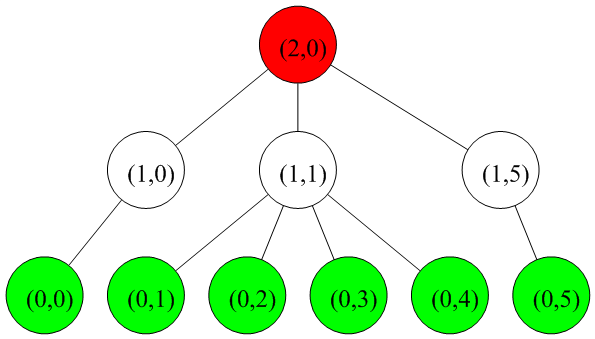
\includegraphics[width=.55\linewidth]{criticalassessment/criticalassessment-selection-refinement-a.png}}%
	%
	\\
	%
	\subfigure[After deselecting $(1,1)$]
	{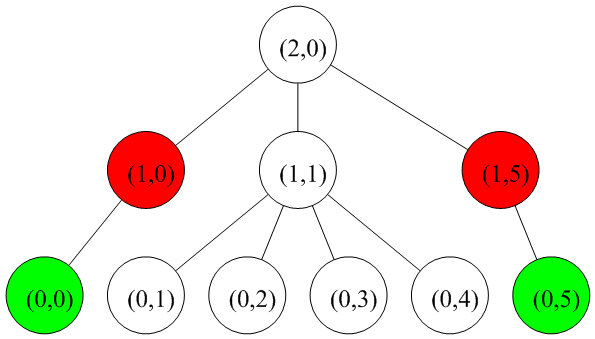
\includegraphics[width=.55\linewidth]{criticalassessment/criticalassessment-selection-refinement-b.png}}%
\caption{Refining the hierarchical representation of a selection (shown in red) is more efficient than refining the flat, leaf-based representation (shown in green)}
\label{fig:criticalassessment-selection-refinement}
\end{stusubfig}
%---

%---
\begin{stusubfig}{p}
	\subfigure[Initial selection]
	{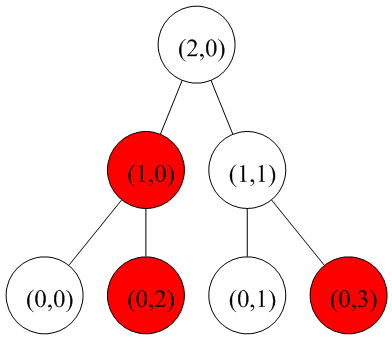
\includegraphics[width=.4\linewidth]{criticalassessment/criticalassessment-selection-redundancy-a.png}}%
	%
	\hspace{4mm}%
	%
	\subfigure[After `deselecting' $(0,2)$]
	{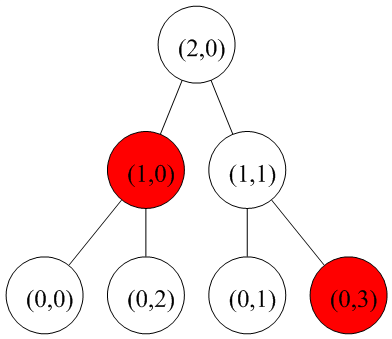
\includegraphics[width=.4\linewidth]{criticalassessment/criticalassessment-selection-redundancy-b.png}}%
\caption{Redundant selection representations can prove confusing to the user -- in this example, it is unclear whether we expect $(0,2)$ to still be selected in (b), since although we have deselected $(0,2)$ itself, it is still implicitly selected as a descendant of $(1,0)$}
\label{fig:criticalassessment-selection-redundancy}
\end{stusubfig}
%---

The core algorithms I have developed to maintain this hierarchical representation are both efficient and practically useful -- in particular, they have been implemented in both the \emph{centipede} and \emph{millipede} systems and allow the user to intuitively manage selections of nodes from multiple layers of a partition forest without any slow-down. The listening algorithms are also interesting, as they ensure that a selection is updated in line with changes to its corresponding partition forest, making it easier to integrate partition forest selections into a graphical user interface.

Whilst the partition forest selection data structure is inherently tied to partition forests themselves, the underlying hierarchical representation and algorithms are fully transferable to other partition hierarchies, including even non-complete partition trees. It would be easy, for example, to use the ideas here to represent the selection of parts of a binary space partitioning (BSP) tree, as used for spatial representation in some 3D games (perhaps as part of a program that depicted the BSP representation of a world visually to aid understanding). The selection algorithms thus have applications beyond the limited confines of my doctorate.

\iffalse
+ Usefulness well-justified
+ Algorithms carefully pinned down, reasonable complexities
+ No comparison in the literature
+ Can be reused for feature marking
\fi

%##################################################################################################
\section{New Waterfall Algorithm}
%##################################################################################################

In \S\ref{subsubsec:segmentation-waterfall-myalgorithm}, I described a new tree-based algorithm I developed for the waterfall transform, based on a similarly tree-based waterfall algorithm developed by my colleague Chris Nicholls \cite{nicholls09}. Nicholls' algorithm was designed to be far easier to implement than the reference algorithm we already had available, due to Marcotegui \cite{marcotegui05}, and in particular to lend itself well to implementation in a functional programming language such as Haskell. In this, it achieves its aims brilliantly -- even my C++ implementation of Nicholls' algorithm only required roughly $100$ lines of code, and Chris's implementation in Haskell is even shorter. In addition to being easy to implement, Nicholls' algorithm is also efficient, running in linear time once the initial minimum spanning tree has been constructed.

One slight downside of both the Nicholls and Marcotegui algorithms is in how they handle non-minimal plateaux in the minimum spanning tree on which the algorithms work. Specifically, Nicholls' algorithm produces results that depend on where the minimum spanning tree is rooted (and on the order of the children at each node), and Marcotegui's algorithm produces results that depend on the internal implementation of the priority queue used.

My goal in developing a new algorithm was to make its results invariant to such implementation details. The new algorithm has the following advantages:
%
\begin{itemize}
\item It produces consistent results for any given minimum spanning tree.
\item Like Nicholls' algorithm, it is reasonably easy to implement and runs in linear time.
\item Because it carefully classifies the edges in the minimum spanning tree into different types, it is very useful when implementing other waterfall algorithms -- in particular, I was able to make use of it when implementing the first step of Marcotegui's algorithm.
\end{itemize}

\newpage

\noindent There are still some downsides, however:
%
\begin{itemize}
\item Most notably, whilst the algorithm produces consistent results for a given minimum spanning tree, it \emph{cannot} produce consistent results for the graph from which the minimum spanning tree was constructed (this is a general problem for all minimum spanning tree-based implementations, including both the Nicholls and Marcotegui algorithms). The results of the algorithm thus still depend on which minimum spanning tree was constructed from the graph. There is no way around this other than to revert to a slower, graph-based implementation.
\item Whilst the algorithm is still linear, it requires a constant factor more work than Nicholls' algorithm, as it has to perform more than one pass of the tree.
\item The algorithm is somewhat harder to implement than Nicholls' algorithm, although it is still relatively easy to code.
\end{itemize}
%
For these reasons, Nicholls' algorithm is still a generally preferable way of performing a waterfall transform, except when the original graph is known to have only one possible minimum spanning tree (for instance, because it itself is a tree) and consistent handling of minimal plateaux is desired.

\iffalse
# Based on Chris's work
+ Produces results that do not depend on the implementation of key data structures (like Marcotegui's) or where the MST is rooted (like Chris's)
+ Efficient, linear-time algorithm
+ Useful as a first step in other waterfall algorithms, because it carefully pins down the types of different edges
+ Easy to implement
- Produces results that depend on which MST is constructed (all MST-based algorithms, including Chris's, necessarily do this -- the only alternative is to run the waterfall on a graph and accept that it will be slower)
- Requires a constant factor more work than Chris's
- Not as easy to implement as Chris's
- The 'incorrect' version of Chris's actually produces better results than either this one or Chris's 'correct' version(!)
\fi

%##################################################################################################
\section{Partition Forest Construction}
%##################################################################################################

In \S\ref{sec:segmentation-ipfconstruction}, I described two separate algorithms for constructing partition forests from 3D image volumes. Both algorithms work in a bottom-up fashion\footnote{Recall from \S\ref{sec:background-partitionhierarchies} that top-down methods tend to produce incomplete partition hierarchies, making them less suitable here.} and construct a single partition forest for the entire image. The \emph{volume-at-once} method does this by hierarchically segmenting the entire image volume using morphological watershed and waterfall algorithms. The \emph{subvolume} method, by contrast, conceptually divides the image volume up into equally-sized pieces, segments each one separately and combines the results. This has the advantage of allowing individual slices to be segmented separately using 2D segmentation techniques.

There are a number of partition forest construction methods in the literature (e.g.~\cite{yu02,marfil07}) -- as with my algorithms, they all work bottom-up. Unlike my approaches, they were generally designed with 2D rather than 3D images in mind, but the techniques required are not substantively different. A good example is the method of Yu et al.\ \cite{yu02}, which starts with a leaf layer whose nodes correspond to small $4 \times 4$ or $8 \times 8$ blocks of pixels in an underlying 2D image. Each node is accorded a vector of region properties that depend on the values and locations of the pixels of the node's corresponding region in the image. Each edge of the adjacency graph representing a layer is weighted with the Euclidean distance between the property vectors of the nodes it joins. In order to construct each new layer, a disjoint set forest (see \S\ref{sec:appendixds-dsf}) is created from the adjacency graph of the current top-most layer. The idea is to decide which nodes should be merged to form the new layer, keeping track of the process using the efficient set-combining operation provided by the disjoint set forest. The decision as to which nodes to merge is based on their region properties. First, we merge (in the disjoint set forest) any pair of nodes connected by an edge whose weight is less than a user-specified threshold (in other words, nodes whose region property vectors are considered sufficiently similar). Second, we find each node in the current top-most layer that has not yet been merged with another node, and merge it with its most similar neighbour -- this is done to ensure fast convergence of the algorithm. Having chosen which nodes to merge, we then construct a new layer by effectively cloning the current top-most layer and combining the nodes as specified by the disjoint set forest. The process terminates either when the current top-most layer contains only one node, or based on a user-specified stop criterion.

A direct comparison between the results of the various construction methods is not especially meaningful, in that they all produce different partition forests (they are not all trying to solve the same problem), but they all follow the general bottom-up approach of constructing each new layer by segmenting the previous one. In that sense, my volume-at-once method has a great deal in common with existing algorithms. The major differences between the algorithms are:
%
\begin{itemize}

\item The segmentation techniques used -- approaches like those in \cite{yu02} and \cite{marfil07} make local decisions about which regions to merge at each stage based on inter-region similarity, whereas my approach segments the current top-most layer using a waterfall pass, which is a global segmentation technique.

\item The way in which new layers are constructed -- my implementation clones the existing top-most layer and then merges some of the regions together, whereas existing methods, such as that in \cite{yu02}, tend to first determine which nodes should be merged and to then construct the new top-most layer explicitly (in much the same way that I construct the lowest branch layer explicitly in \S\ref{subsec:segmentation-ipfconstruction-volumeatonce}). My implementation approach has the advantage of making it possible to avoid explicitly propagating graph edges from the current top-most layer to the new layer being added above it.

\end{itemize}
%
In all other respects, however, the volume-at-once method is a relatively conventional approach to partition forest construction, albeit that it works on 3D rather than 2D images.

The subvolume method, on the other hand, is distinctly different from previous algorithms. Whilst the 2D algorithms in the literature transfer readily enough to 3D, it can still sometimes be desirable (for reasons already outlined) to segment individual 2D slices through a 3D image separately. Existing algorithms (having been designed with only 2D images in mind) do not allow us to do this -- as such, the subvolume method fills an important niche.

Both of my forest construction methods could benefit from more efficient implementation, as will be discussed in \S\ref{sec:conclusions-furtherwork}. The majority of the time currently spent in constructing forests is taken up by preprocessing the input image (since anisotropic diffusion filtering is quite a slow process) -- it would be helpful to explore ways in which this could be parallelized to speed things up. Additionally, the subvolume method as currently implemented requires substantial additional storage space during the construction process, and it would be good to find a way of minimizing the amount of memory required.

\iffalse
+ Subvolume method works for both 2D and 3D segmentation
+ Need to compare both methods to the literature
- Both methods are relatively slow, primarily because of the significant preprocessing time required (anisotropic diffusion filtering, at least as implemented in ITK, is slow as hell)
- Construction process uses twice as much memory as the finished partition forest
\fi

%##################################################################################################
\section{Feature Identification Techniques}
%##################################################################################################

In Chapter~\ref{chap:featureid}, I described a number of 2D and 3D techniques for identifying abdominal features. The 3D identifiers in particular were quantitatively validated in Chapter~\ref{chap:validation}, whilst the 2D spine identifier was qualitatively assessed in the original paper that introduced it \cite{gvcispa09}.

%################################################
\subsection{2D Identification Techniques}
%################################################

TODO

%################################################
\subsection{3D Identification Techniques}
%################################################

TODO

\iffalse
+ The feature identifiers are relatively quick to run
+ The 2D ribs identifier is relatively effective, although it can miss ribs in some cases
+ The 2D spine identifier is effective and robust (about 85\% of results are pretty good)
+ The 3D spine identifier is relatively effective and robust, but has a tendency to flood into the ribs a bit
+ The 3D spinal canal identifier is relatively effective and robust, although the contour of the spinal canal is by no means perfect yet
+ The 3D kidneys identifier is a reasonable start, but requires further work both to make it more robust and to detect kidneys that are made up of multiple regions 
- Because the current techniques are based on region growing, they suffer from the usual sort of region growing problems; a better approach might be to use the partition forest to find initial features, and then use level sets
- The 3D aorta identifier only works well when the segmentation is particularly good; it needs further work
- The 3D liver identifier is not ideal (although it does start out in the right place), and has a tendency to flood into other features
\fi

%##################################################################################################
\section{Implementation}
%##################################################################################################

As mentioned in the introduction, over the course of my doctorate I developed two separate segmentation, feature identification and visualization systems, called \emph{centipede} and \emph{millipede}. Each of these was a substantial, medium-sized system -- as a rough\footnote{I am aware that lines of code is a somewhat unreliable way of measuring the size of a project, but it does at least allow us to distinguish between small, medium and large projects.} indication of scale, \emph{centipede} (the trial system) had $26000+$ lines of C++ code, and \emph{millipede} (the final system) $32000+$ lines. Additionally, \emph{millipede} was designed to be a highly portable, cross-platform project built using CMake -- to date, it has been successfully used on Microsoft Windows, Linux (Ubuntu) and Mac OS X (Snow Leopard), but it is potentially portable to other platforms as well.

The two systems make a vital contribution to this thesis, because they demonstrate that the approach actually works in practice, and on widely-available consumer hardware. From the perspective of future developers, \emph{millipede} in particular also provides a consistently-designed and easily-maintainable code-base that forms a firm foundation for further research work. The build process has been carefully documented on all three of the platforms mentioned, allowing other developers to pick up the project and make changes without the Herculean struggle often associated with building unfamiliar code.

In terms of assessing the development process itself, the development of \emph{millipede} proceeded far more smoothly than that of \emph{centipede}, for a number of reasons:
%
\begin{enumerate}

\item \textbf{Better Domain Knowledge}. Most importantly, \emph{millipede} was developed with the difficulties of developing \emph{centipede} firmly in mind, which allowed me to avoid many of the pitfalls I had encountered the first time around, whilst delivering a more feature-rich end result. (A few examples of specific improvements were that (a) I was able to redesign my partition forest implementation to be faster and more coherent, (b) I was able to implement segmentation and feature identification in 3D as well as 2D, and (c) I was able to make the user interface more responsive using multithreading.)

\item \textbf{Better Tools}. When developing \emph{centipede}, I made the mistake of insisting on developing my own underlying imaging toolkit rather than using the `off-the-shelf' alternative\footnote{In industry, this folly is commonly referred to as suffering from the `not invented here' syndrome.}, which resulted in the initial development taking far longer than it otherwise would have done; for \emph{millipede}, I chose to use the \emph{Insight Toolkit} (ITK) instead.

\item \textbf{Better Scheduling}. The development of \emph{millipede} progressed under much tighter time constraints than \emph{centipede}, which forced me to construct a much more focused development plan, keeping only essential features and avoiding `feature creep'. The actual time spent on implementing \emph{millipede} itself was roughly six months, compared to roughly a year overall for \emph{centipede}.

\end{enumerate}
%
The lessons I have taken from this are that:
%
\begin{enumerate}

\item It is important to build a trial system, but it is often a good idea to then ditch that trial system and start again with the benefit of hindsight. (This echoes Fred Brooks' well-known advice of `Plan to throw one away; you will, anyhow.' \cite{brooks74}) In this case, rewriting from scratch was by far the best option (if a slightly frustrating one from a development perspective), because it allowed improvements to be made that would have taken far longer to integrate into the existing \emph{centipede} system.

\item It is especially crucial to avoid reinventing the wheel when developing systems of a non-trivial size. The goal of learning more about how things work by redeveloping them yourself is a worthwhile one, but that must not be done during the development of a system that has real-world time constraints. Redoing work that has already been done by somebody else takes time away from new work. Systems you redevelop yourself are also often less reliable than their `off-the-shelf' counterparts, which have been subjected to significant testing in the real world.

\item Having less time can result in a better end result, because you are forced to develop only what is necessary. However, this can only work when you already know what you are developing (which is not usually the case at the start of a research project).

\end{enumerate}

\iffalse
+ Medium-size systems (30k+ lines of code each)
+ Implementation of millipede carefully planned with feature list -- very functional, but no unnecessary 'bells and whistles' / feature creep
+ The implementation of millipede proceeded rapidly and according to schedule
+ Consistent, maintainable code (particularly millipede)
+ millipede is entirely cross-platform -- built using CMake; works on Windows, Linux and Mac
+ Runs on normal consumer desktops / laptops
- Should have used ITK the first time round (instead of suffering from NIH syndrome)
- Should have written centipede to be cross-platform from the start
\fi

%##################################################################################################
\section{Chapter Summary}
%##################################################################################################

In this chapter, each of the original contributions mentioned in the introduction was critically assessed. The final chapter contains some concluding remarks and pinpoints some opportunities for further work.
